% Options for packages loaded elsewhere
\PassOptionsToPackage{unicode}{hyperref}
\PassOptionsToPackage{hyphens}{url}
%
\documentclass[
]{article}
\usepackage{amsmath,amssymb}
\usepackage{iftex}
\ifPDFTeX
  \usepackage[T1]{fontenc}
  \usepackage[utf8]{inputenc}
  \usepackage{textcomp} % provide euro and other symbols
\else % if luatex or xetex
  \usepackage{unicode-math} % this also loads fontspec
  \defaultfontfeatures{Scale=MatchLowercase}
  \defaultfontfeatures[\rmfamily]{Ligatures=TeX,Scale=1}
\fi
\usepackage{lmodern}
\ifPDFTeX\else
  % xetex/luatex font selection
\fi
% Use upquote if available, for straight quotes in verbatim environments
\IfFileExists{upquote.sty}{\usepackage{upquote}}{}
\IfFileExists{microtype.sty}{% use microtype if available
  \usepackage[]{microtype}
  \UseMicrotypeSet[protrusion]{basicmath} % disable protrusion for tt fonts
}{}
\makeatletter
\@ifundefined{KOMAClassName}{% if non-KOMA class
  \IfFileExists{parskip.sty}{%
    \usepackage{parskip}
  }{% else
    \setlength{\parindent}{0pt}
    \setlength{\parskip}{6pt plus 2pt minus 1pt}}
}{% if KOMA class
  \KOMAoptions{parskip=half}}
\makeatother
\usepackage{xcolor}
\usepackage[margin=1in]{geometry}
\usepackage{graphicx}
\makeatletter
\def\maxwidth{\ifdim\Gin@nat@width>\linewidth\linewidth\else\Gin@nat@width\fi}
\def\maxheight{\ifdim\Gin@nat@height>\textheight\textheight\else\Gin@nat@height\fi}
\makeatother
% Scale images if necessary, so that they will not overflow the page
% margins by default, and it is still possible to overwrite the defaults
% using explicit options in \includegraphics[width, height, ...]{}
\setkeys{Gin}{width=\maxwidth,height=\maxheight,keepaspectratio}
% Set default figure placement to htbp
\makeatletter
\def\fps@figure{htbp}
\makeatother
\setlength{\emergencystretch}{3em} % prevent overfull lines
\providecommand{\tightlist}{%
  \setlength{\itemsep}{0pt}\setlength{\parskip}{0pt}}
\setcounter{secnumdepth}{-\maxdimen} % remove section numbering
\ifLuaTeX
  \usepackage{selnolig}  % disable illegal ligatures
\fi
\usepackage{bookmark}
\IfFileExists{xurl.sty}{\usepackage{xurl}}{} % add URL line breaks if available
\urlstyle{same}
\hypersetup{
  pdftitle={Hedging Against Turkish Inflation},
  pdfauthor={Selin Acar, Necati Furkan Çolak, Denis Lasser},
  hidelinks,
  pdfcreator={LaTeX via pandoc}}
\usepackage{graphicx}
\usepackage{natbib}
\usepackage{hyperref}

\title{Hedging Against Turkish Inflation}
\author{Selin Acar, Necati Furkan Çolak, Denis Lasser}
\date{December 2024}

\begin{document}
\maketitle

{
\setcounter{tocdepth}{2}
\tableofcontents
}
\pagebreak

\section{Introduction}\label{introduction}

The ongoing economic crisis in Türkiye has been characterized by high
inflation, the depreciation of the Turkish Lira (TRY), rising borrowing
costs, and increasing loan defaults. The underlying causes of the crisis
can be attributed to several factors, including political instability,
global economic pressures, and the implementation of unconventional
economic policies. Since 2018, inflation has been a persistent issue,
partly due to fluctuations in global oil prices and exchange rates, with
Turkey's inflation rate ranking among the highest in emerging markets
\citet{yilmazkuday_2022}. The effectiveness of inflation-targeting policies
has been limited by both internal shocks, such as political events and
the COVID-19 pandemic, and external factors, such as rising global
inflation \citep{nazlioglu_2024}.Furthermore, the Turkish
government's policy of maintaining low interest rates to stimulate
growth, despite the conventional theory that raising interest rates
should reduce inflation, has contributed significantly to the current
economic challenges \citep{kantur_ozcan_2021}. Nevertheless, interest
rates have been raised significantly. As of November 2024, the most
recent rate hike was in March 2024, when the central bank increased the
policy rate by 5 percentage points to 50\% as the year-on-year inflation
reached 75\% \citep{bloomberg_2024}. Since then, the rate has remained
unchanged as the central bank has been committed to fighting high
inflation and stabilising the Turkish lira. As of October 2024,
year-on-year inflation stands at 48\% \citep{bloomberg_2024}. This study aims
to analyze which assets, as well as which portfolio of assets, would
have been the most effective in hedging against Turkish inflation.

\section{Methodology}\label{methodology}

This study examines the effectiveness of various assets as hedges
against Turkish inflation, using monthly data from January 2018 to
September 2024. The monthly frequency was selected for the following
reasons:

\begin{enumerate}
\def\labelenumi{\arabic{enumi}.}
\tightlist
\item
  The use of monthly data allows for the smoothing of short-term
  fluctuations. This facilitates the identification of more coherent
  relationships between inflation and asset returns.
\item
  Key economic indicators, including inflation rates, are typically
  reported on a monthly basis. By aligning asset data with this
  frequency, the analysis maintains consistency and relevance in
  relation to reported inflation rates.
\item
  The influence of short-term trading anomalies, seasonal effects and
  temporary market shocks on weekly data must be acknowledged. Monthly
  data minimizes the impact of these irregularities, thereby providing a
  more stable basis for the analysis of assets as potential inflation
  hedges.
\end{enumerate}

\subsection{Data Collection}\label{data-collection}

This study includes a range of assets to capture different potential
hedging mechanisms against inflation.

Following indices were sourced from Bloomberg:

\begin{itemize}
\item
  \textbf{TUCXEFYY Index}: This index tracks the Turkish CPI (Consumer
  Price Index) excluding categories such as food, energy, alcohol, and
  tobacco. This represents the core inflation rate and excludes the most
  volatile components of the CPI, given that the aforementioned
  categories are often subject to short-term price fluctuations due to
  external factors. In the context of hedging against inflation, it is
  more meaningful to focus on core inflation, as short-term fluctuations
  in volatile categories can distort the true underlying inflation rate.
  Therefore, this index serves as the benchmark and allows for direct
  comparison of the other assets against inflation.
\item
  \textbf{XU100 Index} (BIST 100): This index comprises the 100 largest
  companies traded at the Borsa Istanbul and provides insight into the
  response of Turkish stocks to inflation.
\item
  \textbf{GTTRY10YR} (10-Year Turkish Government Bond): Long-term
  government bonds, such as the 10-year Turkish government bond, are
  traditionally considered low-risk investments. Including this bond in
  the analysis allows for an assessment of the inflation risk premium
  embedded in Turkish government debt.
\item
  \textbf{XAU}: This index represents the price of one ounce of gold
  quoted in US Dollars (USD). Gold is often seen as a traditional hedge
  against inflation due to its historical retention of value. Analyzing
  gold prices in USD allows for an assessment of gold's ability to
  preserve purchasing power during periods of high inflation in Türkiye,
  while avoiding the potential distortions caused by exchange rate
  volatility.
\item
  \textbf{XBT BGN}: Bitcoin is included in the analysis as an
  alternative inflation hedge, with prices analyzed in USD. Analyzing
  Bitcoin in USD focuses on its performance as a global inflation hedge,
  independent of potential distortions caused by exchange rate
  volatility. This approach provides insights into Bitcoin's ability to
  preserve purchasing power and its relevance in the context of Turkish
  inflation.
\end{itemize}

Furthermore, the house price index data was obtained from the Turkish
Central Bank's EVDS database
(\url{https://evds2.tcmb.gov.tr/index.php?/evds/portlet/KSAktmjeowo\%3D/en}).
Specifically, the \textbf{TP KFE TR-1} series was used, which tracks
nationwide residential property price change in Türkiye. Real estate is
often considered a strong inflation hedge, as property values and rental
income tend to rise with inflation. This index allows an analysis of the
effectiveness of the real estate sector in preserving purchasing power
during inflationary periods.

\subsection{Analysis Techniques}\label{analysis-techniques}

The analysis consists of two main steps. First, the effectiveness of
each individual asset in providing a hedge is evaluated. Subsequently,
an optimal hedging portfolio is determined.

The first step is to calculate the \textbf{excess return} for each asset
relative to the Turkish inflation rate.

This calculation differs depending on whether the asset is denominated
in TRY or USD:

\begin{itemize}
\tightlist
\item
  Asset denominated in TRY:
\end{itemize}

\[
\text{Excess Return}= \text{Nominal Return} - \text{Inflation Rate}
\]

Excess return is calculated as the asset's return minus the Turkish
inflation rate over the same period. This straightforward calculation
reflects the direct impact of inflation on TRY-denominated assets.

\begin{itemize}
\tightlist
\item
  Asset denominated in USD:
\end{itemize}

\[
\text{Excess Return} = \frac{1 + \text{Nominal Return}}{1 + \text{Inflation Rate}} - 1
\]

In this case, Turkish inflation is used to adjust the nominal return.
Real returns for USD-denominated assets, such as gold and Bitcoin, are
calculated using Turkish inflation rates to assess their effectiveness
in preserving purchasing power in Türkiye. While nominal returns in USD
account for global factors, real returns adjusted for Turkish inflation
provide a clearer measure of an asset's ability to hedge against the
specific inflationary pressures experienced in Türkiye.

This first step evaluates each asset's ability to preserve purchasing
power. Assets with consistently positive excess returns are considered
to have stronger hedging characteristics, as they maintain or increase
purchasing power above inflation. This initial analysis provides a basis
for assessing each asset's stand-alone ability to serve as an inflation
hedge.

Building on the individual asset analysis, the next step applies
\textbf{Markowitz portfolio optimization} to construct an optimal
portfolio that maximizes the hedging effectiveness against Turkish
inflation. Markowitz optimization, also referred to as
\textbf{Mean-Variance Optimization}, determines the portfolio
composition that achieves the highest return for a given level of risk /
the lowest risk for a given return. In the context of this study, the
aim is to construct a portfolio that minimizes inflation risk while
providing stable excess returns. By balancing a range of assets,this
optimization creates a portfolio that preserves purchasing power against
inflation more effectively than any individual asset alone.

The process involves the following calculations:

\begin{enumerate}
\def\labelenumi{\arabic{enumi}.}
\tightlist
\item
  \textbf{Portfolio Return}: \[
  \text{Portfolio Return} = R_p = \sum_{i=1}^{n} w_i R_i
  \]
\end{enumerate}

where:

\begin{itemize}
\tightlist
\item
  \(R_p\): Portfolio return
\item
  \(w_i\): Weight of asset \(i\) in the portfolio
\item
  \(R_i\): Return of asset \(i\)
\item
  \(n\): Number of assets in the portfolio
\end{itemize}

\begin{enumerate}
\def\labelenumi{\arabic{enumi}.}
\setcounter{enumi}{1}
\tightlist
\item
  \textbf{Portfolio Variance}: \[
  \text{Portfolio Variance} = \sigma_p^2 = \sum_{i=1}^{n} \sum_{j=1}^{n} w_i w_j \sigma_{ij}
  \]
\end{enumerate}

where:

\begin{itemize}
\tightlist
\item
  \(\sigma_p^2\): Portfolio variance (measure of risk)
\item
  \(w_i, w_j\): Weights of assets \(i\) and \(j\) in the portfolio
\item
  \(\sigma_{ij}\): Covariance between the returns of assets \(i\) and
  \(j\)
\item
  \(\sigma_{ii}\) or \(\sigma_i^2\): Variance of asset \(i\) (case when
  \(i = j\)
\end{itemize}

\begin{enumerate}
\def\labelenumi{\arabic{enumi}.}
\setcounter{enumi}{2}
\tightlist
\item
  \textbf{Minimizing Portfolio Risk}: \[
  \min_{w} \, \sigma_p^2 \quad \text{subject to:} \quad \sum_{i=1}^{n} w_i R_i = R_{\text{target}}, \quad \sum_{i=1}^{n} w_i = 1, \quad w_i \geq 0
  \]
\end{enumerate}

where:

\begin{itemize}
\tightlist
\item
  \(\min_{w} \, \sigma_p^2\): The objective is to minimize the portfolio
  variance
\item
  \(\sum_{i=1}^{n} w_i R_i = R_{\text{target}}\): The portfolio must
  achieve a specified target return (\(R_{\text{target}}\))
\item
  \(\sum_{i=1}^{n} w_i = 1\): The sum of portfolio weights must equal 1,
  this ensures that the portfolio is fully invested
\item
  \(w_i \geq 0\): Weights must be non-negative, assuming no
  short-selling
\end{itemize}

Solving the optimization problem generates the efficient frontier, which
represents the set of optimal portfolios that offer the highest return
for a given level of risk. The efficient frontier is derived by varying
\(R_{\text{target}}\) and solving the optimization problem for each
level of return.

\section{Results}\label{results}
\subsection{Real Return of Individual Assets}
\textbf{a) Turkish Stocks}

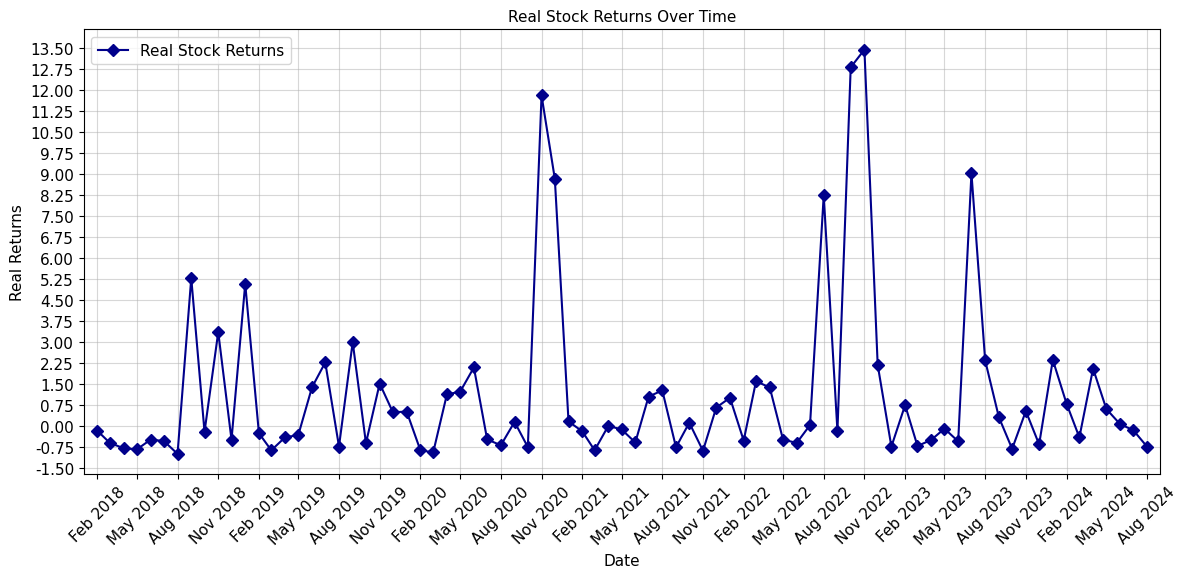
\includegraphics[width=\textwidth]{figures/real-returns-stocks.png}

Turkish stocks are highly volatile, with several sharp peaks and troughs. For instance, there are noticeable spikes in returns, especially around mid-2020 and mid-2021.

Therefore, Turkish equities appear to offer opportunities for inflation hedging during certain periods, but are inconsistent as a hedge. While they may reflect market optimism during inflationary periods, they still carry significant risks, as shown by the high volatility.

\textbf{b) Turkish Government Bond}

\includegraphics[width=\textwidth]{figures/real-returns-gov-bonds.png}

CHECK!!

\textbf{c) Gold}

\includegraphics[width=\textwidth]{figures/real-returns-gold.png}

Gold has traditionally been seen as an inflation hedge. With a real return that has frequently been above 0 over the past six years, these results support this view. Its relative stability, occasional spikes and limited periods of negative real returns suggest that gold can act as a safeguard against inflationary pressures in Turkey. However, short-term fluctuations show that its performance may not always guarantee positive real returns in every period.

\textbf{d) Bitcoin}

\includegraphics[width=\textwidth]{figures/real-returns-bitcoin.png}

Bitcoin's real returns are highly volatile, with several periods of sharp negative and positive returns. Therefore, it is not a consistent hedge against Turkish inflation due to its high volatility. While it offers occasional large positive returns, it also carries significant downside risk. This makes it speculative rather than a stable store of value in the context of inflation hedging.

\textbf{e) Turkish Real Estate}

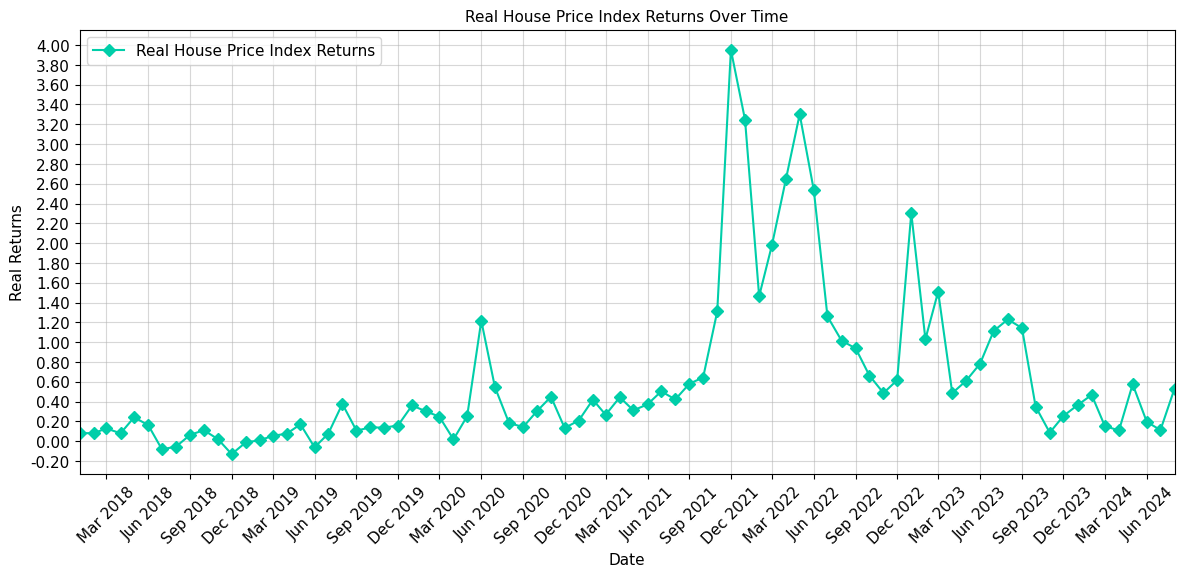
\includegraphics[width=\textwidth]{figures/real-returns-hpi.png}

Turkish real estate showed relative stability in real returns until around 2020, after which there was a sharp increase. The peak in real returns occurred in late 2021, likely driven by a spike in inflation, with real estate acting as a safe haven. Consequently, real estate appears to be a viable hedge against inflation during periods of high inflation in Türkiye The sharp increase in real returns suggests strong investor demand for real assets to preserve wealth amid economic uncertainty.

\subsection{Markowitz Portfolio Optimization}

\section{Conclusion}\label{conclusion}

TEXT TEXT TEXT

\pagebreak

\section{References}
\bibliographystyle{plainnat}
\bibliography{/Users/selin/UZH_Master/HS24/digital-tools/reports/resources}

\end{document}
